\section*{Результаты}
	
\addcontentsline{toc}{section}{Результаты}

	На данный момент сделана программа для анализа периодических сигналов, поиска значимых гармоник и их аппроксимация для дальнейшего нахождения пика QPO. Также сравнены данные по MAXI J1820+070, полученные с инструментов Konus-Wind, Swift/BAT, INTEGRAL/ISGRI, что можно увидеть ниже. Интересно то, что, несмотря на одинаковый спектр одинаковых фотонов у ISGRI и Konus-Wind, счет фотонов после пика у них разный. В конце работы будут получены зависимости амплитуды и частоты пульсирующей компоненты сигнала от времени для Vela-X1, GX301-2, A0535+262, SWIFT J0243.6+6124 и эволюция параметров QPO для MAXI1820+070.
	
	\begin{figure}[h!]
		\begin{subfigure}[b]{0.45\textwidth}
			\centering
			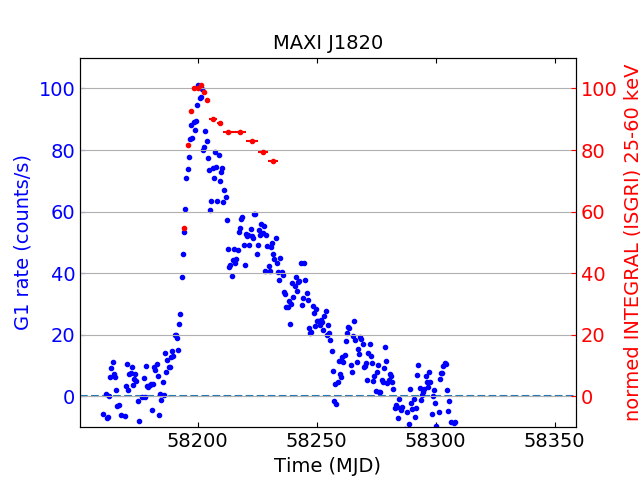
\includegraphics[width=\textwidth]{pictures/MAXIJ1820_kwG1_int.png}
			\caption{}
		\end{subfigure}
		\begin{subfigure}[b]{0.45\textwidth}
			\centering
			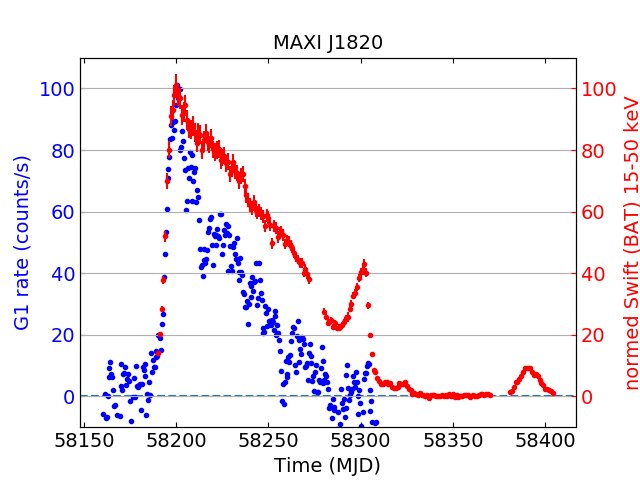
\includegraphics[width=\textwidth]{pictures/MAXIJ1820_kwG1_bat.png}
			\caption{}				
		\end{subfigure}
		\caption{Сравнение счета фотонов у Конус-Винд c (a) INTEGRAL или (b) BAT}
	\end{figure}

\newpage

\addcontentsline{toc}{section}{Список литературы}
\bibliography{all}
